\documentclass{beamer}

\usepackage[utf8]{inputenc}
\usepackage[french]{babel}
\usepackage{graphicx}

\title{Présentation Git \& Github}
\author{Eliesse HADJEM}

\usetheme[secheader]{Madrid}


\begin{document}

  \begin{frame}
    \maketitle
  \end{frame}
  
  \begin{frame}
    \tableofcontents
  \end{frame}

\section{La gestion de version}
\subsection{Concept}
\begin{frame}
 \frametitle{Une problématique}
    Comment permettre aux utilisateurs de partager l'information, tout en les empêchant de se marcher dessus ?
    \begin{figure}
 \centering
 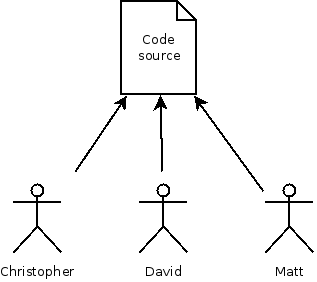
\includegraphics[width=50mm]{./Img/AccesConc.png}
 % AccesConc.png: 0x0 pixel, 0dpi, 0.00x0.00 cm, bb=
 \caption{Différents Docteurs veulent acceder à la source}
\end{figure}


\end{frame}
\begin{frame}
 \frametitle{Une solution}
  \framesubtitle{La gestion de version (ou Version Control)}
    \begin{quote}
     La gestion de version consiste à maintenir l'ensemble des version d'un ou plusieurs fichier. 
    \end{quote}
    \begin{figure}
 \centering
 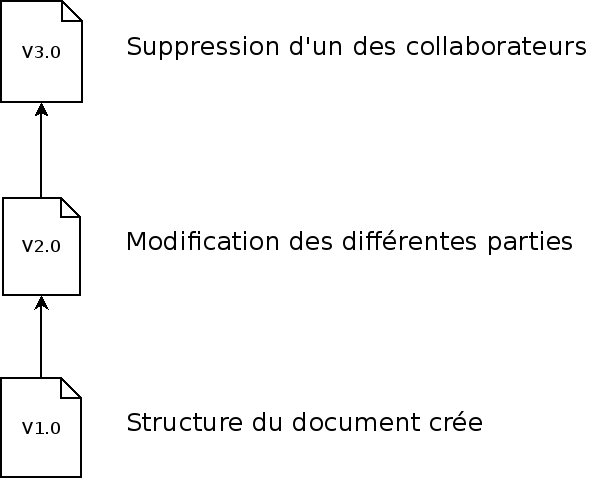
\includegraphics[width=50mm]{./Img/VersionsFich.png}
 % Diagramme1.png: 0x0 pixel, 0dpi, 0.00x0.00 cm, bb=
 \caption{Différentes version d'un fichier}
\end{figure}
    
\end{frame}

\begin{frame}
\frametitle{Une solution}
  \framesubtitle{Le gestionnaire de version}
   Un gestionnaire de version est un système qui enregistre l'évolution d'un fichier au cours du temps.\\
   Ce système permet de récupérer à tout moment une version antérieure du fichier.
\end{frame}

\begin{frame}
 \frametitle{Une solution}
 \framesubtitle{Exemple}
\begin{figure}
 \centering
 \includegraphics[width=10mm]{./Diagramme1.png}
 % Diagramme1.png: 0x0 pixel, 0dpi, 0.00x0.00 cm, bb=
 \caption{Différentes version d'un fichier}
\end{figure}
\end{frame}



\subsection{Notions}
\begin{frame}
\frametitle{Les types de gestionnaires de version}
\begin{itemize}
 \item Les gestionnaires centralisés : CVS, SVN
 \item Les gestionnaires décentralisés : GNU Arch, Mercurial, Git
\end{itemize}
\end{frame}


\begin{frame}
\frametitle{Version}
La version d'un fichier est l'avancement des modification d'un fichier qui a été validé par l'utilisateur.
\end{frame}

\begin{frame}
\frametitle{Branche}
Une branche est une version d'un projet que l'on souhaite continuer de manière indépendante 
\end{frame}


\section{Git}

\section{Github}
\begin{frame}
 Lol
\end{frame}


\end{document}